\providecommand{\main}{../../..}
\documentclass[\main/dresen_thesis.tex]{subfiles}
\renewcommand{\thisPath}{\main/chapters/appendix/additionalExperimentalTechniques}
\begin{document}

\chapter{Additional Instruments}
\section{PPMS - Vibrating Sample Magnetometry}
\label{app:additionalExperimentalTechniques:vsm}
For vibrating sample magnetometry, a dispersion of nanoparticles is enclosed in a sealed container and brought to vibration with a specific frequency.

\section{Bruker D8 - X-Ray Reflectometry}
\label{app:additionalExperimentalTechniques:xrr}
\begin{figure}[h]
  \centering
  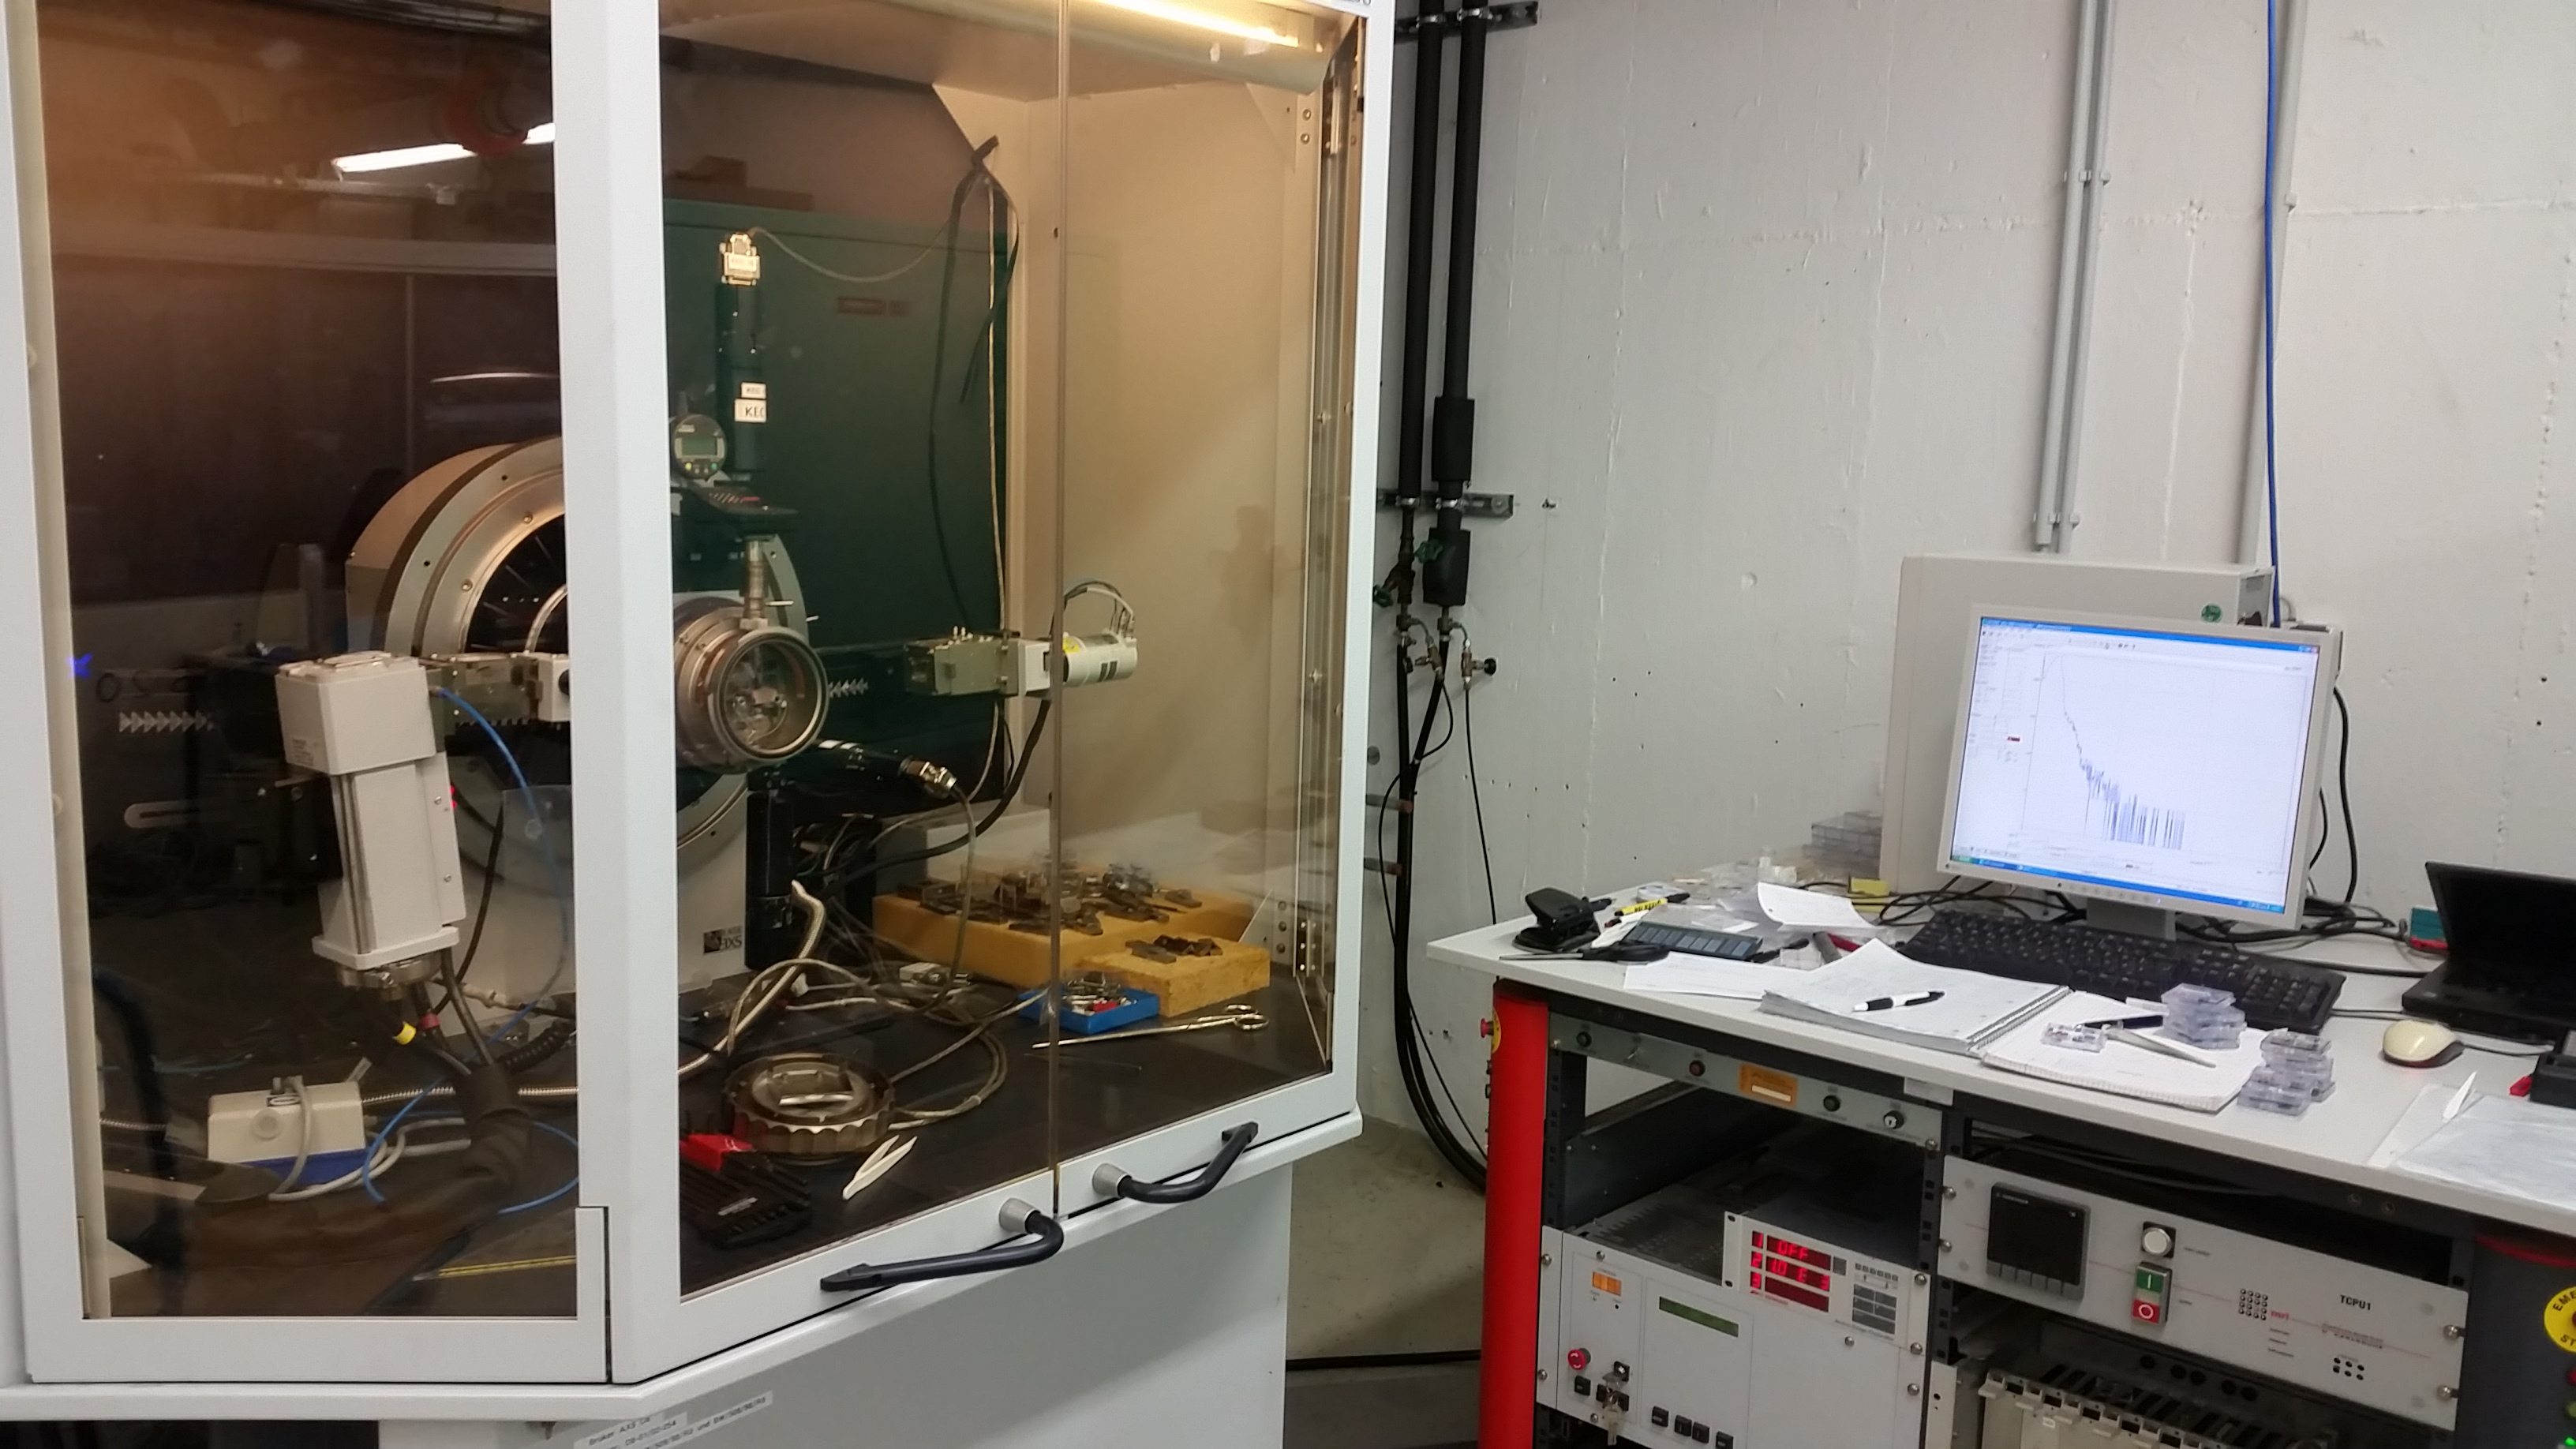
\includegraphics[width=0.7\textwidth]{instruments_brukerD8}
  \caption{\label{fig:appendix:instruments:brukerD8}Bruker D8 instrument which can be used for x-ray reflectometry and x-ray diffraction.}
\end{figure}
To study the vertical structure of thin-layer samples, x-ray reflectometry (XRR) is a quick method. In this work, multiple samples were studied with XRR using the \textsc{Bruker D8} instrument in the \textsc{Forchungszentrum J\"ulich}.
For XRR, the incident angle of the beam and the outgoing angle are increased simultaneously to maintain the specular condition while scanning the reflected intensity over $q_z$.
The beam size can be varied by slits and is typically set to $0.2 \unit{mm}$.
To estimate the beam divergence, the direct beam is scanned with the detector in \reffig{fig:appendix:instruments:brukerD8DirectBeam}.
The best fit with a gaussian function results in a divergence of $\Delta \alpha_i \eq 0.01510(4) ^\circ \eq 2.635(7) \cdot 10^{-4}.$
\begin{figure}[tb]
  \centering
  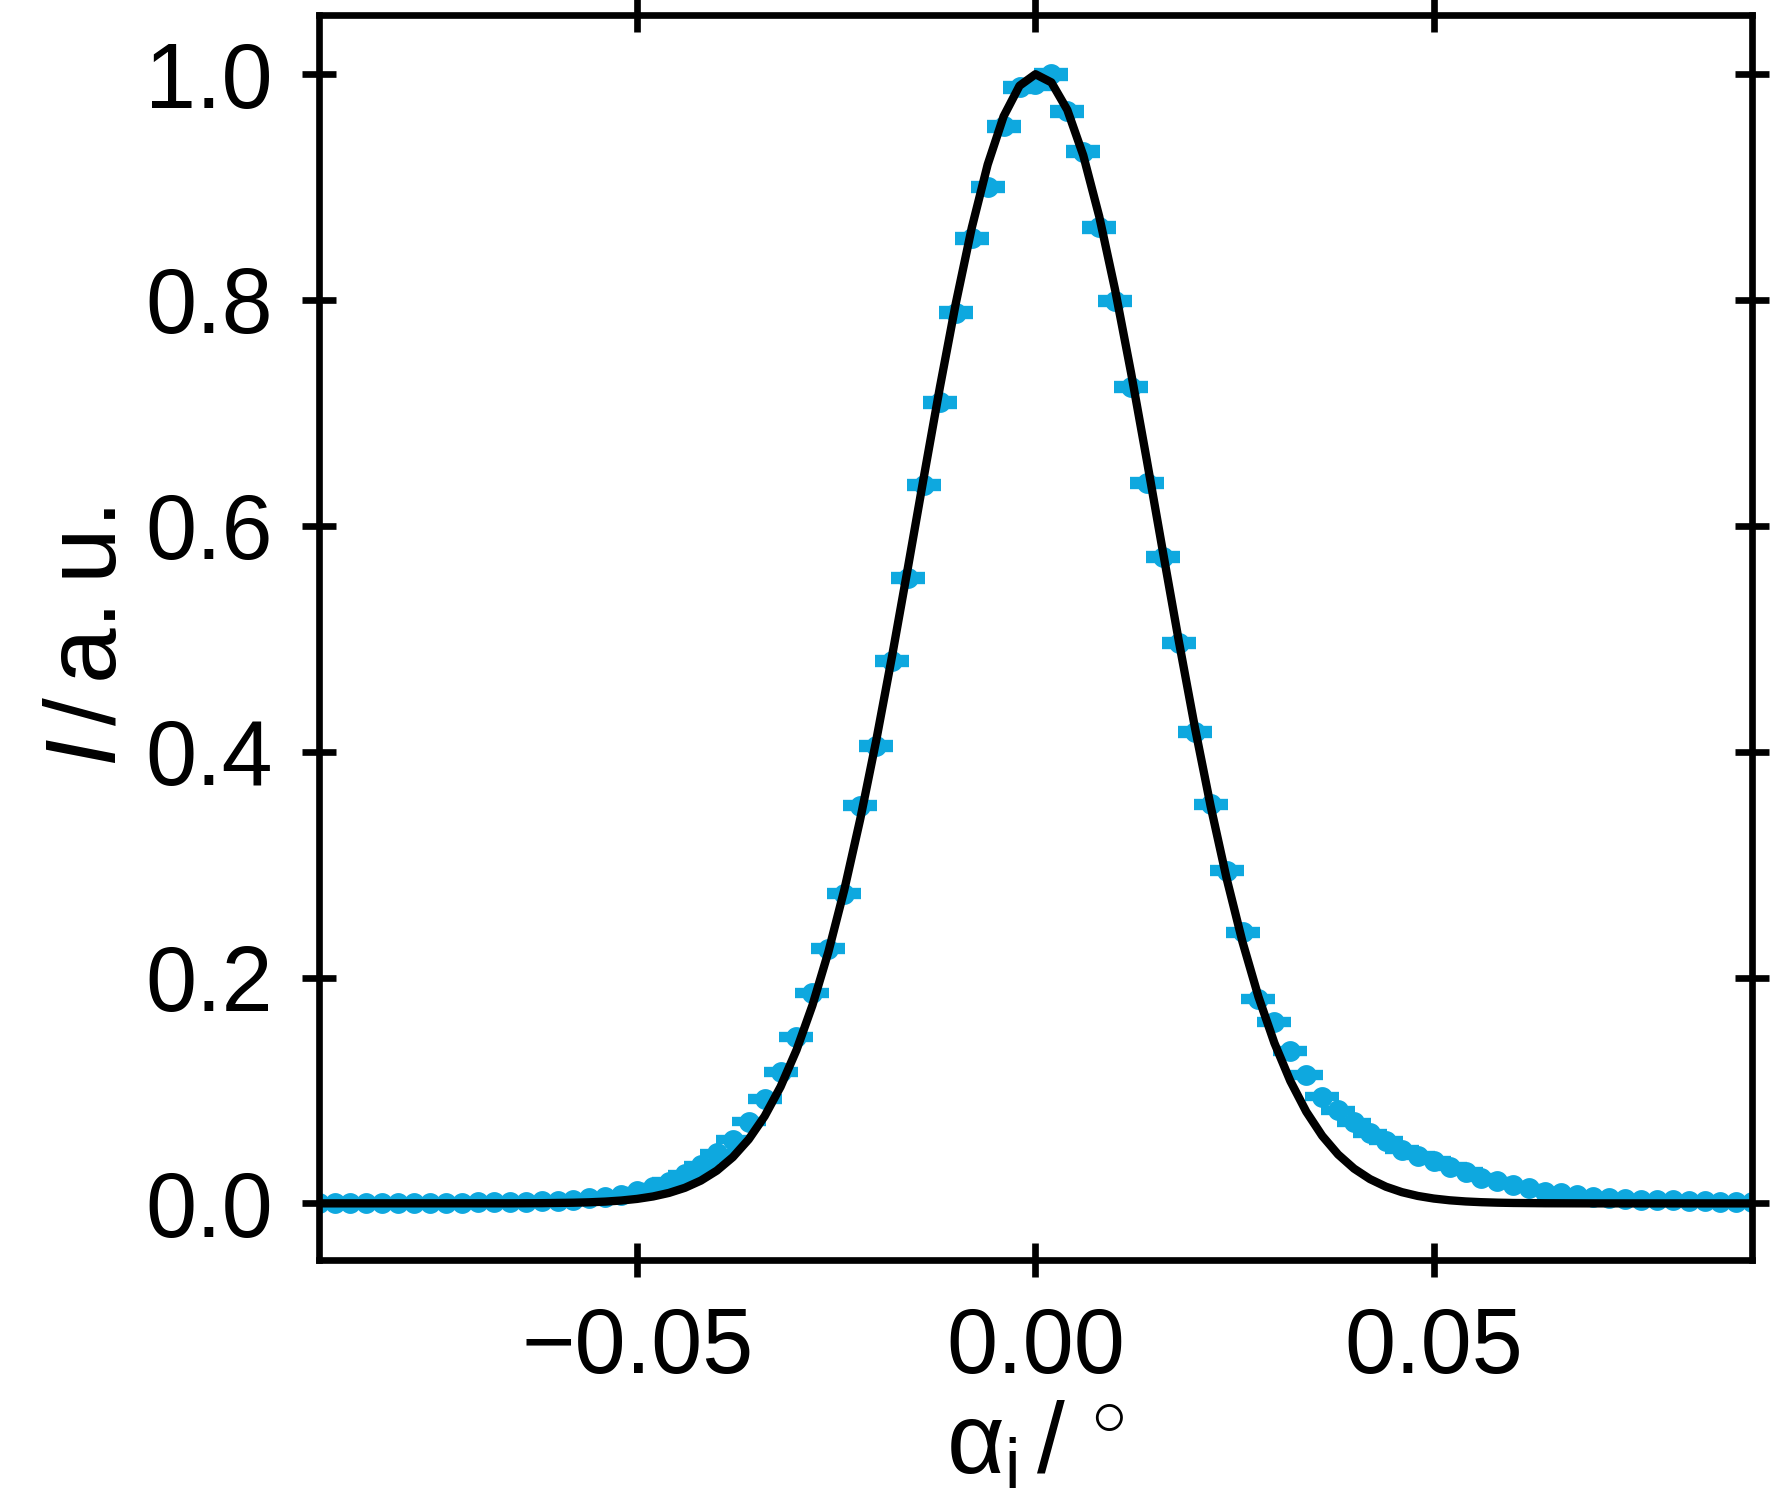
\includegraphics{appendix_instruments_brukerD8DirectBeam}
  \caption{\label{fig:appendix:instruments:brukerD8DirectBeam}Direct beam scan of the Bruker D8 instrument at a beam slit size of $0.2 \unit{mm}$, modelled by a gaussian function to estimate the divergence.}
\end{figure}
\end{document}
